\documentclass[10pt,a4paper]{article}
\usepackage[margin=25mm]{geometry}
\usepackage{amsmath,amssymb,amsthm,graphicx,hyperref}
\title{Pointed connected coverings are classified by subgroups of the fundamental group in homotopy type theory}
\author{Samuel Mimram, Émile Oleon}
\date{doi:10.4230/LIPIcs.CSL.2026.21; CC BY4.0 (official published text and diagrams)}
\begin{document}
\maketitle
\noindent\textit{Editorial note.} Copyright Samuel Mimram and Émile Oleon; official CSL2026.21, CC BY4.0. One pointed-connected-covering/subgroup classification theorem; its support/inverse directions and existing generated/presented-group delooping background do not add counts.\par\medskip
\noindent\textit{Allowed standard prerequisites (editorial).}\begin{itemize}
\item Standard HoTT truncation, long exact homotopy sequence, Grothendieck action/fibration duality and delooping background. Original paper bibliography including HoTT book and generated/presented-group delooping sources; existing lane LL022/LL023 are background only. Full current Galois-fibration and new classification/fiber proofs are actually retained.
\end{itemize}\medskip

% BEGIN S2
 
\par\medskip\noindent\textbf{2 Homotopy type theory}\par
 
% BEGIN S2.p1
 
We begin by briefly recalling the main notations and tools of homotopy type theory. Detailed presentations can be found in [14, 12].\par
 
% END S2.p1
 
% BEGIN S2.SS0.SSS0.P0.SPx1
 
\par\medskip\noindent\textbf{Universe.}\par
 
% BEGIN S2.SS0.SSS0.P0.SPx1.p1
 
We write $\mathcal{U}$ for the universe type, whose elements are small types, which is supposed to be closed under dependent sum and product types. Given a type $A:\mathcal{U}$ and a type family $B:A\to\mathcal{U}$, we write $\Sigma A.B$ or $\Sigma(x:A).B\,x$ for dependent sum types and $\Pi A.B$ or $\Pi(x:A).B\,x$ or $(x:A)\to B\,x$ for dependent product types. As customary, we respectively write $A\times B$ and $A\to B$ for product and arrow types, which correspond to non-dependent particular cases of the previous constructions. We respectively write $0$ and $1$ for the initial and terminal types.\par
 
% END S2.SS0.SSS0.P0.SPx1.p1
 
% END S2.SS0.SSS0.P0.SPx1
 
% BEGIN S2.SS0.SSS0.P0.SPx2
 
\par\medskip\noindent\textbf{Identities.}\par
 
% BEGIN S2.SS0.SSS0.P0.SPx2.p1
 
The type theory features a notion of definitional equality and we write $t\equiv u$ when two terms $t$ and $u$ are definitionally equal. It also features a notion of propositional equality: given $x,y:A$, we write $x=y$ for the type of identities or paths between $x$ and $y$ in $A$. For any point $x:A$, there is a path $\operatorname{refl}:x=x$ witnessing reflexivity. Given paths $p:x=y$ and $q:y=z$, we can construct paths $p\cdot q:x=z$ corresponding to concatenation or transitivity, and $p^{-1}:y=x$ corresponding to inverse or symmetry.\par
 
% END S2.SS0.SSS0.P0.SPx2.p1
 
% END S2.SS0.SSS0.P0.SPx2
 
% BEGIN S2.SS0.SSS0.P0.SPx3
 
\par\medskip\noindent\textbf{Pointed types.}\par
 
% BEGIN S2.SS0.SSS0.P0.SPx3.p1
 
A pointed type is a type $A$ together with a distinguished element, often written $\star_{A}$ or even $\star$ (equivalently, the distinguished element can be specified by providing a map $1\to A$). A pointed map $f:A\to B$ between pointed types $A$ and $B$ is a map between the underlying types together with an identification $f(\star_{A})=\star_{B}$. We write $A\to_{\star{}}B$ for the corresponding type of pointed maps.\par
 
% END S2.SS0.SSS0.P0.SPx3.p1
 
% END S2.SS0.SSS0.P0.SPx3
 
% BEGIN S2.SS0.SSS0.P0.SPx4
 
\par\medskip\noindent\textbf{Univalence.}\par
 
% BEGIN S2.SS0.SSS0.P0.SPx4.p1
 
A map $f:A\to B$ is an equivalence when it admits both a left and a right inverse. We write $A\simeq B$ for the type of equivalences between $A$ and $B$. Any identity between two types canonically induces an equivalence between them. The univalence axiom states that the corresponding map $(A=B)\to(A\simeq B)$ is itself an equivalence: in particular, any equivalence induces an identity.\par
 
% END S2.SS0.SSS0.P0.SPx4.p1
 
% END S2.SS0.SSS0.P0.SPx4
 
% BEGIN S2.SS0.SSS0.P0.SPx5
 
\par\medskip\noindent\textbf{Homotopy levels.}\par
 
% BEGIN S2.SS0.SSS0.P0.SPx5.p1
 
A type $A$ is contractible when it is equivalent to $1$. A type $A$ is a proposition (resp. a set, resp. a groupoid) when for any elements $x,y:A$ the type $x=y$ is contractible (resp. a proposition, resp. a set). The type of sets is denoted $\operatorname{Set}$. More generally, we can define a notion of $n$-type for $n\in\left\{-2,-1\right\}\cup\mathbb{N}$ by stating that a $(-2)$-type is a contractible one, and an $(n{+}1)$-type is a type $A$ in which $x=y$ is an $n$-type for every $x,y:A$. We write $\operatorname{isType}_{n}(A)$ for the predicate indicating that $A$ is an $n$-type, which can be shown to be a proposition. We write $\mathcal{U}_{n}\equiv\Sigma\mathcal{U}.\operatorname{isType}_{n}$ for the type of $n$-types.\par
 
% END S2.SS0.SSS0.P0.SPx5.p1
 
% END S2.SS0.SSS0.P0.SPx5
 
% BEGIN S2.SS0.SSS0.P0.SPx6
 
\par\medskip\noindent\textbf{Truncation.}\par
 
% BEGIN S2.SS0.SSS0.P0.SPx6.p1
 
The $n$-truncation $\|A\|_{n}$ is the universal way of turning a type $A$ into an $n$-type: it comes equipped with a map $|{-}|_{n}:A\to\|A\|_{n}$ such that any map $f:A\to B$, whose target $B$ is an $n$-type, induces a unique map $\tilde{f}:\|A\|_{n}\to B$ such that $\tilde{f}(|x|_{n})=f(x)$ for $x:A$. A type $A$ is $n$-connected when $\|A\|_{n}=1$. In particular, a type is connected (resp. simply connected) when it is $0$-connected (resp. $1$-connected). The connected component of an element $a$ of $A$ is $\Sigma(x:A).\|a=x\|_{-1}$.\par
 
% END S2.SS0.SSS0.P0.SPx6.p1
 
% END S2.SS0.SSS0.P0.SPx6
 
% BEGIN S2.SS0.SSS0.P0.SPx7
 
\par\medskip\noindent\textbf{Loop space.}\par
 
% BEGIN S2.SS0.SSS0.P0.SPx7.p1
 
The circle $\operatorname{S}^{1}$ is the free pointed type containing a path $\operatorname{loop}:\star=\star$. Given a pointed type $A$, its loop space $\operatorname{\Omega}A$ is $\star=\star$, which can be shown to coincide with the type $\operatorname{S}^{1}\to_{\star{}}A$. Its fundamental group is the type $\pi_{1}(A)\equiv\|\operatorname{\Omega}A\|_{0}$, which is canonically equipped with a group structure induced by path concatenation. When $A$ is a pointed connected groupoid, its loop space coincides with its fundamental group, so that it is a group. A delooping of a group $G$ is a type $\operatorname{B}G$ equipped with an isomorphism of groups $\operatorname{\Omega}\operatorname{B}G\cong G$ (such a type always exists and is unique, thus the notation). It is easily shown that a map $\operatorname{B}G\to\operatorname{Set}$ corresponds to a set equipped with an action of $G$ in the usual sense.\par
 
% END S2.SS0.SSS0.P0.SPx7.p1
 
% END S2.SS0.SSS0.P0.SPx7
 
% BEGIN S2.SS0.SSS0.P0.SPx8
 
\par\medskip\noindent\textbf{Fiber sequences.}\par
 
% BEGIN S2.SS0.SSS0.P0.SPx8.p1
 
Given a map $f:A\to B$ and $y:B$, the fiber of $f$ at $y$ is the type $\operatorname{fib}_{f}y\equiv\Sigma(x:A).(f(x)=y)$. When $B$ is pointed, the kernel of $f$ is $\ker f\equiv\operatorname{fib}_{f}\star$. A composable pair of morphisms 
\begin{center}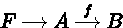
\includegraphics[width=0.95\linewidth,height=0.45\textheight,keepaspectratio]{graphic-01.pdf}\end{center}
 is a fiber sequence when $F$ is the kernel of $f$ and the map $F\to A$ is the first projection. A map is $n$-connected (resp. $n$-truncated) when all its fibers are.\par
 
% END S2.SS0.SSS0.P0.SPx8.p1
 
% END S2.SS0.SSS0.P0.SPx8
 
% BEGIN S2.SS0.SSS0.P0.SPx9
 
\par\medskip\noindent\textbf{The Grothendieck duality.}\par
 
% BEGIN S2.SS0.SSS0.P0.SPx9.p1
 
A fundamental property in homotopy type theory is that, given a type $A$, fibrations over $A$ correspond both to types over $A$ and to type families indexed by $A$: this is the Grothendieck duality. We write $\mathcal{U}/A\equiv\Sigma(B:\mathcal{U}).(B\to A)$ for the type of types over $A$ and $A\to\mathcal{U}$ for the type of type families indexed by $A$. We have a function $\operatorname{fib}:\mathcal{U}/A\to(A\to\mathcal{U})$, which to $p:B\to A$ associates the fiber $\operatorname{fib}_{p}:A\to\mathcal{U}$, and a function $\int:(A\to\mathcal{U})\to(\mathcal{U}/A)$, which to a family $F:A\to\mathcal{U}$ associates the first projection map $\pi:\Sigma A.F\to A$. The following is shown in [14, Section 4.8]:\par
 
% END S2.SS0.SSS0.P0.SPx9.p1
 
% BEGIN Thmtheorem1
 
\par\medskip\noindent\textbf{Theorem 1.}\par
 
% BEGIN Thmtheorem1.p1
 
Given a type $A$, the above functions induce an equivalence $\mathcal{U}/A\simeq(A\to\mathcal{U})$. Moreover, this correspondence is functorial in the sense that given $p:B\to A$ and $q:C\to A$, a morphism $f:B\to C$ with $q\circ f=p$ corresponds to a family of maps $(x:A)\to\operatorname{fib}_{p}x\to\operatorname{fib}_{q}x$ in a way which preserves identities and composition (and thus equivalences).\par
 
% END Thmtheorem1.p1
 
% END Thmtheorem1
 
% END S2.SS0.SSS0.P0.SPx9
 
% END S2


% BEGIN S3
 
\par\medskip\noindent\textbf{3 Higher covering types}\par
 
% BEGIN S3.SS1
 
\par\medskip\noindent\textbf{3.1 Covering spaces in topology}\par
 
% BEGIN S3.SS1.p1
 
We briefly recall here the traditional notion of covering space in topology and refer to standard textbooks for details [7]. Given a topological space $A$, a covering is a space $B$ together with a map $p:B\to A$ which is locally trivial. This means that every point $x:B$ admits an open neighborhood such that the preimage $p^{-1}(U)$ is homeomorphic to a space of the form $U\times F$, where $F$ is a set equipped with the discrete topology and the restriction of $p$ to $p^{-1}(U)$ is the first projection. When $B$ is connected, which will be the case of interest here, the cardinal of $F$ has to be the same for every point $x$ and is called the number of sheets of the covering. Below we have figured a covering with 3 sheets (on the left) and with countably many sheets (on the right):\par
 
\begin{center}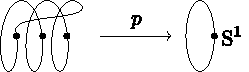
\includegraphics[width=0.95\linewidth,height=0.45\textheight,keepaspectratio]{graphic-02.pdf}\end{center}

\begin{center}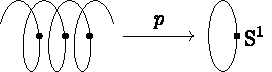
\includegraphics[width=0.95\linewidth,height=0.45\textheight,keepaspectratio]{graphic-03.pdf}\end{center}
 
In order for the constructions of coverings to be well-behaved, we will implicitly assume in the following that $A$ satisfies reasonable assumptions (namely being connected, locally path-connected, semilocally simply-connected). We will also assume that it comes equipped with a distinguished point $\star$. An important feature of coverings is that they have the path lifting property: given a path $\pi:x\rightsquigarrow y$ in $A$ and an element $\tilde{x}\in\tilde{A}$ with $p(\tilde{x})=x$ there is a unique path $\tilde{\pi}:\tilde{x}\to\tilde{y}$ with $p(\tilde{\pi})=\pi$. This implies that we have an action of the fundamental group $\pi_{1}(A)$ on the fiber $p^{-1}(\star)$ and, in fact, this characterizes coverings:\par
 
% END S3.SS1.p1
 
% BEGIN Thmtheorem2
 
\par\medskip\noindent\textbf{Proposition 2 ([7, Section 1.3, p. 70]).}\par
 
% BEGIN Thmtheorem2.p1
 
Coverings of $A$ are in bijection with sets equipped with an action of $\pi_{1}(A)$.\par
 
% END Thmtheorem2.p1
 
% END Thmtheorem2
 
% BEGIN S3.SS1.p2
 
The universal covering is the only covering $p:\tilde{A}\to A$ with $\tilde{A}$ simply connected. For instance, the universal covering of $\operatorname{S}^{1}$ is the “helix” pictured on the right above. This space can be shown to be unique up to isomorphism and can be constructed as follows:\par
 
% END S3.SS1.p2
 
% BEGIN Thmtheorem3
 
\par\medskip\noindent\textbf{Proposition 3 ([7, Section 1.3, p. 64]).}\par
 
% BEGIN Thmtheorem3.p1
 
The universal cover $\tilde{A}$ of $A$ can be constructed as the space whose points are pairs consisting of a point $x:A$ and a path $p:\star\rightsquigarrow x$ up to homotopy, equipped with a suitable topology, the map $p:\tilde{A}\to A$ being given by first projection.\par
 
% END Thmtheorem3.p1
 
% END Thmtheorem3
 
% BEGIN S3.SS1.p3
 
The fundamental group $\pi_{1}(A)$ of $A$ is the group whose elements are homotopy classes of paths $\star\rightsquigarrow\star$ in $A$, with concatenation as multiplication and constant paths as neutral elements. By the construction of Proposition 3, given $x:A$, the fiber $p^{-1}(x)$ is $\pi_{1}(A)$, and we have an action of $\pi_{1}(A)$ on this fiber given by left multiplication, which induces an action of $\pi_{1}(A)$ on $\tilde{A}$.\par
 
% END S3.SS1.p3
 
% BEGIN Thmtheorem4
 
\par\medskip\noindent\textbf{Proposition 4 ([7, Theorem 1.38]).}\par
 
% BEGIN Thmtheorem4.p1
 
The quotient $\tilde{A}/\pi_{1}(A)$ of the universal cover under the above action is precisely $A$.\par
 
% END Thmtheorem4.p1
 
% END Thmtheorem4
 
% BEGIN S3.SS1.p4
 
The action can be shown to be free, so that the quotient above coincides with the homotopy quotient.\par
 
% END S3.SS1.p4
 
% END S3.SS1
 
% BEGIN S3.SS2
 
\par\medskip\noindent\textbf{3.2 The universal fibration}\par
 
% BEGIN S3.SS2.p1
 
We begin by describing a situation in homotopy type theory, which is close to coverings, and fundamental with respect to the characterization of identity types. This construction might seem a bit artificial at first, but we will see that the point of view nicely generalizes to coverings, in the sense that what we describe in this section is a kind of “universal $\infty$-covering”.\par
 
% END S3.SS2.p1
 
% BEGIN S3.SS2.p2
 
Suppose given a pointed type $A$. A pointed type over $A$ is a pointed morphism $p:B\to_{\star{}}A$. A morphism between two such pointed types $p:B\to_{\star{}}A$ and $q:C\to_{\star{}}A$ is a map $f:B\to C$ together with an equality $f\circ p=q$. Such morphisms compose in the expected way, which is compatible with the composition of underlying maps.\par
 
% END S3.SS2.p2
 
% BEGIN Thmtheorem5
 
\par\medskip\noindent\textbf{Definition 5.}\par
 
% BEGIN Thmtheorem5.p1
 
A pointed type $p:B\to_{\star{}}A$ is universal when for every pointed type $q:C\to A$, the type of morphisms from $p$ to $q$ is contractible.\par
 
% END Thmtheorem5.p1
 
% END Thmtheorem5
 
% BEGIN S3.SS2.p3
 
Since it satisfies a universal property, the universal pointed type is unique, and it exists thanks to the following characterization:\par
 
% END S3.SS2.p3
 
% BEGIN Thmtheorem6
 
\par\medskip\noindent\textbf{Proposition 6.}\par
 
% BEGIN Thmtheorem6.p1
 
A pointed type $p:B\to_{\star{}}A$ is universal if and only if $B$ is contractible.\par
 
% END Thmtheorem6.p1
 
% END Thmtheorem6
 
% BEGIN S3.SS2.SSS0.P0.SPx1
 
\par\medskip\noindent\textbf{Proof.}\par
 
% BEGIN S3.SS2.SSS0.P0.SPx1.p1
 
By definition of morphisms and initiality of $1$, the type $1$ is initial among pointed types over $A$. A universal pointed type $p:B\to A$ is also initial among pointed types over $A$, by the universal property, and thus $B$ is equivalent to $1$, i.e. contractible. $\hfill\blacktriangleleft$ By immediate computations, we have:\par
 
% END S3.SS2.SSS0.P0.SPx1.p1
 
% BEGIN Thmtheorem7
 
\par\medskip\noindent\textbf{Proposition 7.}\par
 
% BEGIN Thmtheorem7.p1
 
The fiber of the universal pointed type $p:1\to A$ is $\operatorname{\Omega}A$.\par
 
% END Thmtheorem7.p1
 
% END Thmtheorem7
 
% BEGIN S3.SS2.SSS0.P0.SPx1.p2
 
It is very illuminative to translate the previous definitions and properties under the Grothendieck duality (see Theorem 1). A pointed type over $A$ corresponds to a fibration $P:A\to\mathcal{U}$ together with a distinguished element $\star_{P}$ of $P\star$, and, by Proposition 6, such a fibration is universal precisely when the total space $\Sigma A.P$ is contractible. The universal pointed type thus corresponds to the universal fibration, which is the map $\mathop{\mathcal{F}_{A}}:A\to\mathcal{U}$ defined by $\mathop{\mathcal{F}_{A}}x\equiv(\star=x)$, and pointed by $\operatorname{refl}_{\star}$. By Theorem 1, a morphism between fibrations $P,Q:A\to\mathcal{U}$ corresponds to a family of maps $f:(x:A)\to P\,x\to Q\,x$ together with an identification $f\star\star_{P}=\star_{Q}$. The initiality property of universal pointed types (Definition 5) then translates as the fundamental theorem of identity types [12, Theorem 11.2.2]:\par
 
% END S3.SS2.SSS0.P0.SPx1.p2
 
% BEGIN Thmtheorem8
 
\par\medskip\noindent\textbf{Theorem 8.}\par
 
% BEGIN Thmtheorem8.p1
 
Suppose given a type family $P:A\to\mathcal{U}$ pointed by $\star_{P}:P\,\star$, together with a family of maps\par
  
\par  \quad  \[F:(x:A)\to(\star=x)\to P\,x\]\quad  \quad  
  
and an identification $F\,\star\,\operatorname{refl}_{\star}=\star_{P}$. Then $F$ is a family of equivalences if and only if the total space $\Sigma A.P$ is contractible.\par
 
% END Thmtheorem8.p1
 
% END Thmtheorem8
 
% END S3.SS2.SSS0.P0.SPx1
 
% BEGIN S3.SS2.SSS0.P0.SPx2
 
\par\medskip\noindent\textbf{Proof.}\par
 
% BEGIN S3.SS2.SSS0.P0.SPx2.p1
 
Under the Grothendieck duality of Theorem 1, the type family $P$ corresponds to the pointed type $p:\Sigma A.P\to A$ over $A$, given by the first projection. The family of maps $F$ then corresponds to a morphism between the universal type over $A$ and $p$, i.e. to a pointed map $f:1\to\Sigma A.P$. Then $F$ is a family of equivalences if and only if the induced map $f$ is an equivalence, i.e. if and only if $\Sigma A.P$ is contractible. $\hfill\blacktriangleleft$\par
 
% END S3.SS2.SSS0.P0.SPx2.p1
 
% BEGIN Thmtheorem9
 
\par\medskip\noindent\textbf{$\blacktriangleright$ Remark 9.}\par
 
% BEGIN Thmtheorem9.p1
 
In the situation of the above theorem, the map $P$ can be thought of as being representable, in the sense that $Px=(\star=x)$ (and identities can be thought of as homs in types). This notion was actually used by Voevodsky [15] in order to first define identity types.\par
 
% END Thmtheorem9.p1
 
% END Thmtheorem9
 
% END S3.SS2.SSS0.P0.SPx2
 
% END S3.SS2
 
% BEGIN S3.SS3
 
\par\medskip\noindent\textbf{3.3 Higher covering types}\par
 
% BEGIN S3.SS3.p1
 
We now introduce the notion of $n$-covering type, for any natural number $n$, which can be understood as an $n$-truncated variant of the pointed types of previous section. The traditional notion of covering is the particular case $n=0$, as we indicate in remarks.\par
 
% END S3.SS3.p1
 
% BEGIN S3.SS3.p2
 
An $n$-covering of $A$ is a map $p:B\to A$ whose fibers are $n$-types; such a map is also said to be $n$-truncated. We write\par
  
\par  \quad  \[\operatorname{Covering}_{n}(A)\quad\equiv\quad\Sigma(B:\mathcal{U}).\Sigma(f:B\to A).(x:A).\operatorname{isType}_{n}(\operatorname{fib}_{f}x)\]\quad  \quad  
  
for the type of coverings of $A$. Under the Grothendieck duality, those can also be defined as families of $n$-types.\par
 
% END S3.SS3.p2
 
% BEGIN Thmtheorem10
 
\par\medskip\noindent\textbf{Lemma 10.}\par
 
% BEGIN Thmtheorem10.p1
 
We have an equivalence $\operatorname{Covering}_{n}(A)\simeq(A\to\mathcal{U}_{n})$.\par
 
% END Thmtheorem10.p1
 
% END Thmtheorem10
 
% BEGIN S3.SS3.SSS0.P0.SPx1
 
\par\medskip\noindent\textbf{Proof.}\par
 
% BEGIN S3.SS3.SSS0.P0.SPx1.p1
 
Follows immediately from Grothendieck duality (Theorem 1). $\hfill\blacktriangleleft$\par
 
% END S3.SS3.SSS0.P0.SPx1.p1
 
% BEGIN Thmtheorem11
 
\par\medskip\noindent\textbf{$\blacktriangleright$ Remark 11.}\par
 
% BEGIN Thmtheorem11.p1
 
For $n=0$, we recover the definition covering types of [8, Definition 1], as maps $A\to\operatorname{Set}$. Since $\operatorname{Set}$ is a groupoid [14, Theorem 7.1.11], the universal property of groupoid truncation provides us with an equivalence $(A\to\operatorname{Set})\simeq(\|A\|_{1}\to\operatorname{Set})$. A covering of $A$ thus corresponds to a map $\|A\|_{1}\to\operatorname{Set}$. Moreover, we have by Proposition 30 that $\|A\|_{1}$ is a $\operatorname{B}\pi_{1}A$, from which deduce that a covering of $A$ corresponds to a set equipped with an action of $\pi_{1}A$. We thus recover the traditional Proposition 2, which was formalized in homotopy type theory in [8, Theorem 4].\par
 
% END Thmtheorem11.p1
 
% END Thmtheorem11
 
% BEGIN S3.SS3.SSS0.P0.SPx1.p2
 
A morphism $f$ between $n$-coverings $p:B\to A$ and $q:C\to A$ is a map $f:B\to C$ together with an equality $p=q\circ f$.\par
 
% END S3.SS3.SSS0.P0.SPx1.p2
 
% BEGIN S3.SS3.SSS0.P0.SPx1.p3
 
A pointed $n$-covering is a pointed map $p:B\to_{\star{}}A$ between pointed types, whose underlying map is an $n$-covering. This corresponds exactly to the following notion:\par
 
% END S3.SS3.SSS0.P0.SPx1.p3
 
% BEGIN Thmtheorem12
 
\par\medskip\noindent\textbf{Definition 12.}\par
 
% BEGIN Thmtheorem12.p1
 
A pointed $n$-covering is a factorization\par
  
\par  \quad  
\begin{center}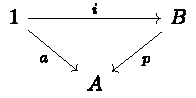
\includegraphics[width=0.95\linewidth,height=0.45\textheight,keepaspectratio]{graphic-04.pdf}\end{center}
\quad  \quad  
  
of the pointing map $a:1\to A$ as $a=p\circ i$ where $p$ is $n$-truncated.\par
 
% END Thmtheorem12.p1
 
% END Thmtheorem12
 
% BEGIN S3.SS3.SSS0.P0.SPx1.p4
 
In the following, we sometimes assimilate the covering to the map $p:B\to A$ leaving the data of the pointing $i:1\to B$ of $B$ implicit. As expected, a morphism $f$ between pointed $n$-coverings $p$ and $q$ is a pointed map which is a morphism between the underlying $n$-coverings, i.e. such that the factorization of the target is $q\circ(f\circ i)$:\par
  
\par  \quad  
\begin{center}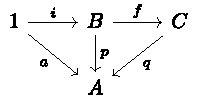
\includegraphics[width=0.95\linewidth,height=0.45\textheight,keepaspectratio]{graphic-05.pdf}\end{center}
\quad  \quad  
  
% END S3.SS3.SSS0.P0.SPx1.p4
 
% BEGIN Thmtheorem13
 
\par\medskip\noindent\textbf{Definition 13.}\par
 
% BEGIN Thmtheorem13.p1
 
A pointed $n$-covering $p:B\to A$ is universal when for every $n$-covering $q:C\to A$ there exists a unique map $f:B\to C$ of pointed $n$-coverings.\par
 
% END Thmtheorem13.p1
 
% END Thmtheorem13
 
% BEGIN Thmtheorem14
 
\par\medskip\noindent\textbf{$\blacktriangleright$ Remark 14.}\par
 
% BEGIN Thmtheorem14.p1
 
For $n=0$, we recover the characterization of pointed universal coverings as being initial in the category of pointed coverings [8, Lemma 12].\par
 
% END Thmtheorem14.p1
 
% END Thmtheorem14
 
% BEGIN S3.SS3.SSS0.P0.SPx1.p5
 
We sometimes write $\tilde{A}$ for the universal $n$-covering. This is justified by the fact that, being defined by a universal property, it is uniquely characterized:\par
 
% END S3.SS3.SSS0.P0.SPx1.p5
 
% BEGIN Thmtheorem15
 
\par\medskip\noindent\textbf{Lemma 15.}\par
 
% BEGIN Thmtheorem15.p1
 
Any two universal pointed $n$-coverings are uniquely isomorphic.\par
 
% END Thmtheorem15.p1
 
% END Thmtheorem15
 
% BEGIN S3.SS3.SSS0.P0.SPx1.p6
 
We have the following characterization of universal $n$-coverings:\par
 
% END S3.SS3.SSS0.P0.SPx1.p6
 
% BEGIN Thmtheorem16
 
\par\medskip\noindent\textbf{Theorem 16.}\par
 
% BEGIN Thmtheorem16.p1
 
Given a pointed type $A$ with pointing map $a:1\to A$, any factorization $a=p\circ i$ as $n$-connected map $i$ and followed by an $n$-truncated map $p$ exhibits $p$ as a universal $n$-covering. Moreover, such a factorization always exists and is unique.\par
 
% END Thmtheorem16.p1
 
% END Thmtheorem16
 
% END S3.SS3.SSS0.P0.SPx1
 
% BEGIN S3.SS3.SSS0.P0.SPx2
 
\par\medskip\noindent\textbf{Proof.}\par
 
% BEGIN S3.SS3.SSS0.P0.SPx2.p1
 
By [14, Theorem 7.6.6], the map $a:1\to A$ admits a unique factorization $a=p\circ i$ as required. Moreover, given a $n$-covering $q:B\to A$ pointed by $b:1\to B$, we have a commuting square as on the left\par
  
\par  \quad   
\begin{center}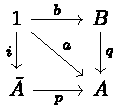
\includegraphics[width=0.95\linewidth,height=0.45\textheight,keepaspectratio]{graphic-06.pdf}\end{center}
 
\begin{center}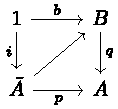
\includegraphics[width=0.95\linewidth,height=0.45\textheight,keepaspectratio]{graphic-07.pdf}\end{center}
 \quad  \quad  
  
The commutation of the two triangles being given by the fact that we have two pointed $n$-coverings of $A$ pointed by $a$. By [14, Theorem 7.6.7], because $i$ is $n$-connected and $p$ is $n$-truncated, there is a unique map $\tilde{A}\to B$ making the two triangles on the right commute, and $p$ is thus universal in the sense of Definition 13. $\hfill\blacktriangleleft$\par
 
% END S3.SS3.SSS0.P0.SPx2.p1
 
% BEGIN S3.SS3.SSS0.P0.SPx2.p2
 
In practice, the universal $n$-covering can be constructed as follows. We recall from [14, Definition 7.6.3] that, given a map $f:B\to A$ and a natural number $n$, its $n$-image is\par
  
\par  \quad  \[\operatorname{im}_{n}f\quad\equiv\quad\Sigma(x:A).\|\operatorname{fib}_{f}x\|_{n}\]\quad  \quad  
  
We write $i_{n}:B\to\operatorname{im}_{n}f$ for the canonical map such that $i_{n}(x)=(f(x),|\operatorname{refl}_{x}|_{n})$ and $p_{n}:\operatorname{im}_{n}f\to A$ for the first projection map.\par
 
% END S3.SS3.SSS0.P0.SPx2.p2
 
% BEGIN Thmtheorem17
 
\par\medskip\noindent\textbf{Proposition 17.}\par
 
% BEGIN Thmtheorem17.p1
 
The factorization $a=p_{n}\circ i_{n}$ of the pointing map $a$ as above, exhibits $p_{n}:\operatorname{im}_{n}a\to A$ as the universal covering of $A$.\par
 
% END Thmtheorem17.p1
 
% END Thmtheorem17
 
% END S3.SS3.SSS0.P0.SPx2
 
% BEGIN S3.SS3.SSS0.P0.SPx3
 
\par\medskip\noindent\textbf{Proof.}\par
 
% BEGIN S3.SS3.SSS0.P0.SPx3.p1
 
By [14, Lemma 7.6.4], this factorization satisfies the conditions of Theorem 16. $\hfill\blacktriangleleft$\par
 
% END S3.SS3.SSS0.P0.SPx3.p1
 
% BEGIN Thmtheorem18
 
\par\medskip\noindent\textbf{$\blacktriangleright$ Remark 18.}\par
 
% BEGIN Thmtheorem18.p1
 
For $n=0$, we recover the usual definition of the universal covering space as the type of homotopy classes of paths from the distinguished point:\par
  
\par  \quad  \[\tilde{A}\quad=\quad\Sigma(x:A).\|\star=x\|_{0}\]\quad  \quad  
  
For $n=-1$, the universal covering of $A$ is its set of connected components. Finally, for $n=\infty$ (we adopt the convention that $\|A\|_{\infty}\equiv A$), we recover the universal pointed type of Section 3.2 by contractibility of singletons [14, Lemma 3.11.8].\par
 
% END Thmtheorem18.p1
 
% END Thmtheorem18
 
% BEGIN Thmtheorem19
 
\par\medskip\noindent\textbf{Example 19.}\par
 
% BEGIN Thmtheorem19.p1
 
The universal covering of $A\equiv\operatorname{S}^{1}$ is $\Sigma(x:A).(\star=x)$ (we can remove the 0-truncation because $\operatorname{S}^{1}$ is a groupoid) and thus contractible by [14, Lemma 3.11.8] (see Lemma 26 for a generalization of this argument).\par
 
% END Thmtheorem19.p1
 
% END Thmtheorem19
 
% BEGIN Thmtheorem20
 
\par\medskip\noindent\textbf{$\blacktriangleright$ Remark 20.}\par
 
% BEGIN Thmtheorem20.p1
 
The factorization results used above hold more generally for any map $a:B\to A$ where $B$ is not necessarily contractible. In this sense, given an arbitrary map $a:B\to A$, we can think of $\operatorname{im}_{n}a$ as the “universal $n$-cover of $A$ relative to $a$”.\par
 
% END Thmtheorem20.p1
 
% END Thmtheorem20
 
% BEGIN S3.SS3.SSS0.P0.SPx3.p2
 
The universal $n$-covering can also be characterized as the covering whose total space is $(n{+}1)$-connected. This can be shown using the following lemma proved in appendix.\par
 
% END S3.SS3.SSS0.P0.SPx3.p2
 
% BEGIN Thmtheorem21
 
\par\medskip\noindent\textbf{Lemma 21.}\par
 
% BEGIN Thmtheorem21.p1
 
A pointed connected type $A$ is $(n{+}1)$-connected (resp. $(n{+}1)$-truncated) if and only if the pointing map $1\to A$ is $n$-connected ($n$-truncated).\par
 
% END Thmtheorem21.p1
 
% END Thmtheorem21
 
% BEGIN Thmtheorem22
 
\par\medskip\noindent\textbf{Theorem 22.}\par
 
% BEGIN Thmtheorem22.p1
 
Given a pointed connected type $A$, the universal pointed $n$-covering is the $(n{+}1)$-connected pointed $n$-covering of $A$.\par
 
% END Thmtheorem22.p1
 
% END Thmtheorem22
 
% END S3.SS3.SSS0.P0.SPx3
 
% BEGIN S3.SS3.SSS0.P0.SPx4
 
\par\medskip\noindent\textbf{Proof.}\par
 
% BEGIN S3.SS3.SSS0.P0.SPx4.p1
 
By Definition 12, a pointed $n$-covering $p:B\to A$ is a factorization of the pointing map $a:1\to A$ as $a=p\circ i$ with $p$ $n$-truncated. By Theorem 16, it is universal if and only if $i:1\to B$ is $n$-connected which, by Lemma 21 is equivalent to the fact that $B$ is $(n{+}1)$-connected. $\hfill\blacktriangleleft$\par
 
% END S3.SS3.SSS0.P0.SPx4.p1
 
% BEGIN Thmtheorem23
 
\par\medskip\noindent\textbf{$\blacktriangleright$ Remark 23.}\par
 
% BEGIN Thmtheorem23.p1
 
For $n=0$, we recover the fact that the universal covering is the only 1-connected covering of a type [8, Lemma 11].\par
 
% END Thmtheorem23.p1
 
% END Thmtheorem23
 
% BEGIN S3.SS3.SSS0.P0.SPx4.p2
 
We now formalize the intuition that the universal $n$-covering $\tilde{A}$ of $A$ provides a way to “kill” all the homotopy in dimension $i\leq n+1$. This is based on what we call the fundamental fibration associated to the universal $n$-covering:\par
 
% END S3.SS3.SSS0.P0.SPx4.p2
 
% BEGIN Thmtheorem24
 
\par\medskip\noindent\textbf{Theorem 24.}\par
 
% BEGIN Thmtheorem24.p1
 
Writing $\tilde{A}$ for the universal $n$-covering, we have a fiber sequence\par
  
\par  \quad  
\begin{center}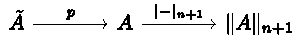
\includegraphics[width=0.95\linewidth,height=0.45\textheight,keepaspectratio]{graphic-08.pdf}\end{center}
\quad  \quad  
  
% END Thmtheorem24.p1
 
% END Thmtheorem24
 
% END S3.SS3.SSS0.P0.SPx4
 
% BEGIN S3.SS3.SSS0.P0.SPx5
 
\par\medskip\noindent\textbf{Proof.}\par
 
% BEGIN S3.SS3.SSS0.P0.SPx5.p1
 
We have\par
  
\par  \quad  \[\ker|{-}|_{n+1}\quad\equiv\quad\Sigma(x:A).(|\star|_{n+1}=|x|_{n+1})\quad=\quad\Sigma(x:A).\|\star=x\|_{n}\quad=\quad\tilde{A}\]\quad  \quad  
  
where middle equality is [14, Theorem 7.3.12] and right one is Proposition 17. $\hfill\blacktriangleleft$ This was actually taken to be the definition of $n$-coverings in [2]. As a corollary, we have the following characterization of the homotopy groups of the universal $n$-covering:\par
 
% END S3.SS3.SSS0.P0.SPx5.p1
 
% BEGIN Thmtheorem25
 
\par\medskip\noindent\textbf{Proposition 25.}\par
 
% BEGIN Thmtheorem25.p1
 
We have $\pi_{i}(\tilde{A})=1$ for $i\leq n+1$ and $\pi_{i}(\tilde{A})=\pi_{i}(A)$ for $i>n+1$.\par
 
% END Thmtheorem25.p1
 
% END Thmtheorem25
 
% BEGIN S3.SS3.SSS0.P0.SPx5.p2
 
In particular, this suggests that the universal covering should be contractible when $A$ has no homotopy in dimension $i>n+1$:\par
 
% END S3.SS3.SSS0.P0.SPx5.p2
 
% BEGIN Thmtheorem26
 
\par\medskip\noindent\textbf{Lemma 26.}\par
 
% BEGIN Thmtheorem26.p1
 
Given a $(n{+}1)$-truncated pointed type $A$, its universal $n$-covering is contractible.\par
 
% END Thmtheorem26.p1
 
% END Thmtheorem26
 
% END S3.SS3.SSS0.P0.SPx5
 
% BEGIN S3.SS3.SSS0.P0.SPx6
 
\par\medskip\noindent\textbf{Proof.}\par
 
% BEGIN S3.SS3.SSS0.P0.SPx6.p1
 
Since $A$ is supposed to be $(n{+}1)$-truncated, the pointing map $a:1\to A$ is $n$-truncated by Lemma 21 and the factorization $a=a\circ\operatorname{id}_{1}$ of the pointing map as an $n$-connected map followed by an $n$-truncated map has to be the factorization of the universal covering (Theorem 16) by uniqueness. $\hfill\blacktriangleleft$\par
 
% END S3.SS3.SSS0.P0.SPx6.p1
 
% BEGIN S3.SS3.SSS0.P0.SPx6.p2
 
We would like to end this section with the following conjecture, which would allow constructing deloopings of higher groups based on the previous construction. Note that, below, the coverings are not supposed to be pointed.\par
 
% END S3.SS3.SSS0.P0.SPx6.p2
 
% BEGIN Thmtheorem27
 
\par\medskip\noindent\textbf{Conjecture 27.}\par
 
% BEGIN Thmtheorem27.p1
 
Given a connected type $A$, the connected component of $\tilde{A}$ in $\operatorname{Covering}_{n}(A)$ is $\|A\|_{n+1}$.\par
 
% END Thmtheorem27.p1
 
% END Thmtheorem27
 
% BEGIN S3.SS3.SSS0.P0.SPx6.p3
 
Provided that this conjecture holds, the connected component of $\tilde{A}$ in $A$ would be a pointed $(n{+}1)$-connected groupoid, which can thus be thought of as a delooping of the fundamental $n$-group of $A$. The following proposition shows that we have right underlying type (it would remain to be shown that we have the right higher operations for the $n$-group):\par
 
% END S3.SS3.SSS0.P0.SPx6.p3
 
% BEGIN Thmtheorem28
 
\par\medskip\noindent\textbf{Proposition 28.}\par
 
% BEGIN Thmtheorem28.p1
 
Given a pointed connected type $A$, the type of automorphisms of the universal $n$-covering $\tilde{A}$ is $\|\operatorname{\Omega}A\|_{n}$.\par
 
% END Thmtheorem28.p1
 
% END Thmtheorem28
 
% END S3.SS3.SSS0.P0.SPx6
 
% BEGIN S3.SS3.SSS0.P0.SPx7
 
\par\medskip\noindent\textbf{Proof.}\par
 
% BEGIN S3.SS3.SSS0.P0.SPx7.p1
 
By universal property of $\tilde{A}$ (Definition 5), an automorphism $f:\tilde{A}\to\tilde{A}$ is uniquely determined by $f\star$ which is an element of $\operatorname{fib}_{p}\star$. The type of automorphisms of $\tilde{A}$ is thus $\operatorname{fib}_{p}\star$. Now, by Proposition 17, we can consider that $p$ is the first projection $p:\Sigma(x:A).\|\operatorname{fib}_{a}x\|_{n}\to A$ whose fiber at $\star$ is $\|\operatorname{fib}_{a}\star\|_{n}$ by [14, Lemma 4.8.1], i.e. $\|\operatorname{\Omega}A\|_{n}$. $\hfill\blacktriangleleft$\par
 
% END S3.SS3.SSS0.P0.SPx7.p1
 
% BEGIN Thmtheorem29
 
\par\medskip\noindent\textbf{$\blacktriangleright$ Remark 29.}\par
 
% BEGIN Thmtheorem29.p1
 
Let us explain why the conjecture does hold in the case $n=0$. Writing\par
  
\par  \quad  \[\operatorname{Comp}(p_{0})\quad\equiv\quad\Sigma(p:\operatorname{Covering}(A)).\|p_{0}=p\|_{-1}\]\quad  \quad  
  
for the connected component of the universal 0-covering $p_{0}:\tilde{A}\to A$, we have\par
  
\par  \quad  \[\operatorname{\Omega}_{p_{0}}\operatorname{Comp}(p_{0})=\operatorname{\Omega}_{p_{0}}\operatorname{Covering}(A)=\|\operatorname{\Omega}A\|_{0}\equiv\pi_{1}(A)\]\quad  \quad  
  
where the first equality follows from the fact that the canonical projection map from $\operatorname{Comp}(p_{0})$ to $\operatorname{Covering}(A)$ is an embedding [14, Lemma 7.6.4], and the second one is due to Proposition 28. Moreover, this identity is compatible with the group structures on both sets.\par
 
% END Thmtheorem29.p1
 
% BEGIN Thmtheorem29.p2
 
Given a group $G$, consider a delooping $A\equiv\operatorname{B}G$. By Grothendieck duality, the type of coverings of $\operatorname{B}G$ coincide with maps $\operatorname{B}G\to\operatorname{Set}$ (see Remark 11), i.e. with the type $\operatorname{Set}_{G}$ of sets equipped with an action of $G$ [8, Theorem 4]. Moreover, under this identification, the universal covering corresponds to the principal $G$-set $P_{G}$, which is the set $G$ equipped with the canonical action induced by right multiplication. Indeed, $\operatorname{B}G$ being a $1$-truncated pointed type, its universal covering is contractible by Lemma 26 and is thus the pointing map $p:1\to\operatorname{B}G$, and the corresponding map $\phi:\operatorname{B}G\to\operatorname{Set}$ is $\phi\equiv\operatorname{fib}_{p}\equiv(x\mapsto\star=x)$. In particular, we have $\phi(\star)=(\star=\star)=\operatorname{\Omega}\operatorname{B}G=G$. Moreover, given an element $a$ of $G$, seen as path $a:\star=\star$, we have $(\phi^{=}a)^{\to}(b)=ab$ by the formula for transport in identity types [14, Lemma 2.11.2]. We thus have that the connected component of the principal $G$-set\par
  
\par  \quad  \[\operatorname{Comp}(P_{G})\equiv\Sigma(X:\operatorname{Set}_{G}).\|P_{G}=X\|_{-1}\]\quad  \quad  
  
is a delooping of $G$. This type is known as the type of $G$-torsors [1, 3, 6, 16].\par
 
% END Thmtheorem29.p2
 
% END Thmtheorem29
 
% END S3.SS3.SSS0.P0.SPx7
 
% END S3.SS3
 
% END S3


% BEGIN S4
 
\par\medskip\noindent\textbf{4 The Galois correspondence}\par
 
% BEGIN S4.SS1
 
\par\medskip\noindent\textbf{4.1 The Galois fibration}\par
 
% BEGIN S4.SS1.p1
 
From now on, we restrict ourselves to the case $n=0$ of $n$-coverings. In order to define the Galois correspondence, we first need to define the action of the fundamental group $\pi_{1}(A)$ of a pointed connected type $A$ on its universal cover $\tilde{A}$. This means that we want to define a map $F:\operatorname{B}\pi_{1}A\to\mathcal{U}$ such that $F\star=\tilde{A}$. By the Grothendieck duality (Theorem 1), this amounts to define a map $f:X\to\operatorname{B}G$, for some type $X$, whose fiber is $\tilde{A}$. Moreover, the source $X$ has to be the homotopy quotient of $\tilde{A}$ under this action, which is known to coincide with the strict quotient because the action is free, and should thus be $A$ itself by Proposition 4, see Section 3.1. Another important observation, is that we have a very convenient model for $\operatorname{B}\pi_{1}A$, namely:\par
 
% END S4.SS1.p1
 
% BEGIN Thmtheorem30
 
\par\medskip\noindent\textbf{Proposition 30.}\par
 
% BEGIN Thmtheorem30.p1
 
Given a pointed connected type $A$, we have that $\|A\|_{1}$ is a $\operatorname{B}\pi_{1}A$.\par
 
% END Thmtheorem30.p1
 
% END Thmtheorem30
 
% BEGIN S4.SS1.SSS0.P0.SPx1
 
\par\medskip\noindent\textbf{Proof.}\par
 
% BEGIN S4.SS1.SSS0.P0.SPx1.p1
 
We take $|\star|_{1}$ to be the distinguished point of $\|A\|_{1}$. Connectedness is preserved by truncation: we have $\|\|A\|_{1}\|_{0}=\|A\|_{0}=1$ (the first equality is [14, Lemma 7.3.15] and the second one is the fact that $A$ is connected) and thus $\|A\|_{1}$ is connected. Finally, we have $\operatorname{\Omega}\|A\|_{1}=\|\operatorname{\Omega}A\|_{0}\equiv\pi_{1}A$ by [14, Corollary 7.3.13]. $\hfill\blacktriangleleft$ The previous discussion suggests defining:\par
 
% END S4.SS1.SSS0.P0.SPx1.p1
 
% BEGIN Thmtheorem31
 
\par\medskip\noindent\textbf{Definition 31.}\par
 
% BEGIN Thmtheorem31.p1
 
Given a pointed connected type $A$, the associated Galois fibration is the map $|-|_{1}:A\to\|A\|_{1}$, which we write $g_{A}$ in the following.\par
 
% END Thmtheorem31.p1
 
% END Thmtheorem31
 
% BEGIN S4.SS1.SSS0.P0.SPx1.p2
 
Its target is $\operatorname{B}\pi_{1}A$ by Proposition 30 and we have the expected fiber as the case $n=0$ of Theorem 24:\par
 
% END S4.SS1.SSS0.P0.SPx1.p2
 
% BEGIN Thmtheorem32
 
\par\medskip\noindent\textbf{Proposition 32.}\par
 
% BEGIN Thmtheorem32.p1
 
We have $\ker g_{A}=\tilde{A}$, i.e. we have a fiber sequence 
\begin{center}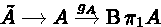
\includegraphics[width=0.95\linewidth,height=0.45\textheight,keepaspectratio]{graphic-09.pdf}\end{center}
.\par
 
% END Thmtheorem32.p1
 
% END Thmtheorem32
 
% BEGIN S4.SS1.SSS0.P0.SPx1.p3
 
As an interesting immediate consequence of this result, we recover the fact that the fibers of the universal covering are the fundamental group:\par
 
% END S4.SS1.SSS0.P0.SPx1.p3
 
% BEGIN Thmtheorem33
 
\par\medskip\noindent\textbf{Proposition 33.}\par
 
% BEGIN Thmtheorem33.p1
 
We have a fiber sequence 
\begin{center}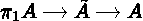
\includegraphics[width=0.95\linewidth,height=0.45\textheight,keepaspectratio]{graphic-10.pdf}\end{center}
.\par
 
% END Thmtheorem33.p1
 
% END Thmtheorem33
 
% END S4.SS1.SSS0.P0.SPx1
 
% BEGIN S4.SS1.SSS0.P0.SPx2
 
\par\medskip\noindent\textbf{Proof.}\par
 
% BEGIN S4.SS1.SSS0.P0.SPx2.p1
 
By [14, Section 8.4], the fiber sequence of Proposition 32 can be extended on the left by $\operatorname{\Omega}\operatorname{B}\pi_{1}A$, which is $\pi_{1}A$ by definition of the delooping. $\hfill\blacktriangleleft$\par
 
% END S4.SS1.SSS0.P0.SPx2.p1
 
% BEGIN S4.SS1.SSS0.P0.SPx2.p2
 
A careful reader could wonder why the action encoded by Proposition 32 is actually the “right” one in the sense that it corresponds to the traditional one in topology. We can expect that there are other such actions, i.e. maps $f:A\to\operatorname{B}\pi_{1}A$ with $\ker f=\tilde{A}$ (what will be important here is that $\tilde{A}$ is 1-connected by Remark 23). In fact, it turns out is only one possible such action, up to an automorphism of $\operatorname{B}\pi_{1}A$:\par
 
% END S4.SS1.SSS0.P0.SPx2.p2
 
% BEGIN Thmtheorem34
 
\par\medskip\noindent\textbf{Proposition 34.}\par
 
% BEGIN Thmtheorem34.p1
 
Given a pointed connected type $A$ and 1-connected map $f:A\to\operatorname{B}\pi_{1}A$, there is an equivalence $e:\operatorname{B}\pi_{1}A\to\operatorname{B}\pi_{1}A$ for which there is a commuting triangle\par
  
\par  \quad  
\begin{center}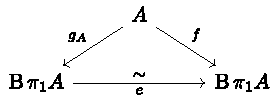
\includegraphics[width=0.95\linewidth,height=0.45\textheight,keepaspectratio]{graphic-11.pdf}\end{center}
\quad  \quad  
  
% END Thmtheorem34.p1
 
% END Thmtheorem34
 
% END S4.SS1.SSS0.P0.SPx2
 
% BEGIN S4.SS1.SSS0.P0.SPx3
 
\par\medskip\noindent\textbf{Proof.}\par
 
% BEGIN S4.SS1.SSS0.P0.SPx3.p1
 
By naturality of truncation [14, equation (7.3.4)], we have a commutative square\par
  
\par  \quad  
\begin{center}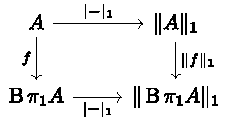
\includegraphics[width=0.95\linewidth,height=0.45\textheight,keepaspectratio]{graphic-12.pdf}\end{center}
\quad  \quad  
  
By definition, the upper map is $g_{A}$. The lower map is $g_{\operatorname{B}\pi_{1}A}$, which is an equivalence because $\operatorname{B}\pi_{1}A$ is a groupoid [14, Corollary 7.3.7]. The right vertical map is also an equivalence by [14, Lemma 7.5.14], because $f$ is supposed to be 1-connected. Finally, $e\equiv g_{\operatorname{B}\pi_{1}A}^{-1}\circ\|f\|_{1}$ is an equivalence as a composite of equivalences. $\hfill\blacktriangleleft$ The situation above is a bit subtle. It states that a 1-connected map as $f$ has to be the Galois fibration. However, this is up to an automorphism of $\operatorname{B}\pi_{1}A$, which might itself bear some information. Indeed, pointed automorphisms of $\operatorname{B}\pi_{1}A$ correspond to group automorphisms of $\pi_{1}A$ which might be non-trivial. In all the applications below, insights from the corresponding constructions in algebraic topology allow us to make sure that we indeed have the right action.\par
 
% END S4.SS1.SSS0.P0.SPx3.p1
 
% END S4.SS1.SSS0.P0.SPx3
 
% END S4.SS1
 
% BEGIN S4.SS2
 
\par\medskip\noindent\textbf{4.2 The Galois correspondence}\par
 
% BEGIN S4.SS2.p1
 
In algebraic topology, we have seen in Proposition 4 that, given a nice pointed space $A$, there is an action of its fundamental group on its universal covering. This is in fact the basis of a classification of (connected) coverings: those correspond to the subgroups of the fundamental group, see for instance [7, Theorem 1.38]. In homotopy type theory, the action is encoded by the Galois fibration (as seen with Proposition 32) and our aim is now to develop a similar classification of coverings. In this section, we write $\operatorname{Covering}(A)$ for the coverings of $A$ which are pointed and connected, i.e. whose total space is connected. Given a group $G$, we also write $\operatorname{Subgroup}(G)$ for the type of subgroups of $G$, i.e. injective maps $i:H\to G$ for some group $H$.\par
 
% END S4.SS2.p1
 
% BEGIN S4.SS2.p2
 
The following lemma, whose proof is provided in appendix, will be useful to show the classification.\par
 
% END S4.SS2.p2
 
% BEGIN Thmtheorem35
 
\par\medskip\noindent\textbf{Lemma 35.}\par
 
% BEGIN Thmtheorem35.p1
 
Given a subgroup $i:H\to G$, the fiber of $\operatorname{B}i$ merely is the set $G/H$.\par
 
% END Thmtheorem35.p1
 
% END Thmtheorem35
 
% BEGIN S4.SS2.p3
 
One of the main results of this paper is the following theorem, see [13] for a formalization:\par
 
% END S4.SS2.p3
 

% BEGIN Thmtheorem36
 
\par\medskip\noindent\textbf{Theorem 36.}\par
 
% BEGIN Thmtheorem36.p1
 
There is an equivalence between subgroups of $\pi_{1}(A)$ and pointed connected coverings of $A$:\par
  
\par  \quad  \[\operatorname{Subgroup}(\pi_{1}(A))\simeq\operatorname{Covering}(A)\]\quad  \quad  
  
% END Thmtheorem36.p1
 
% END Thmtheorem36

 
% BEGIN S4.SS2.SSS0.P0.SPx1
 
\par\medskip\noindent\textbf{Proof.}\par
 
% BEGIN S4.SS2.SSS0.P0.SPx1.p1
 
Given a subgroup $i:G\hookrightarrow\pi_{1}(A)$, the corresponding covering $X$ is obtained as pullback of the Galois fibration along the delooping of group inclusion:\par
  
\par  \quad  
\begin{center}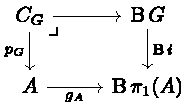
\includegraphics[width=0.95\linewidth,height=0.45\textheight,keepaspectratio]{graphic-13.pdf}\end{center}
\quad  \quad  
  
We need to show that $C_{G}$ is a connected covering, i.e. it is connected and $p_{G}$ has $0$-truncated fibers. The fiber of the covering is given by pasting pullbacks\par
  
\par  \quad  
\begin{center}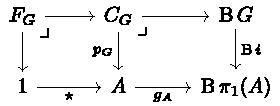
\includegraphics[width=0.95\linewidth,height=0.45\textheight,keepaspectratio]{graphic-14.pdf}\end{center}
\quad  \quad  
  
and thus we have\par
  
\par  \quad  \[F_{G}\equiv\ker{p_{G}}=\ker{\operatorname{B}i}=\pi_{1}(A)/G\]\quad  \quad  
  
by Lemma 35 (to be precise, we only have the existence of such an equality, which is sufficient for our purposes exposed in next sentence). As a consequence, the fibers of $p_{G}$ are sets. Also, by vertical pasting of pullbacks,\par
  
\par  \quad  
\begin{center}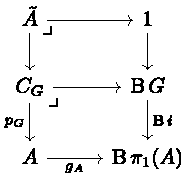
\includegraphics[width=0.95\linewidth,height=0.45\textheight,keepaspectratio]{graphic-15.pdf}\end{center}
\quad  \quad  
  
we have that the upper square is a pullback, i.e. a fibration sequence of the form\par
  
\par  \quad  
\begin{center}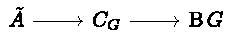
\includegraphics[width=0.95\linewidth,height=0.45\textheight,keepaspectratio]{graphic-16.pdf}\end{center}
\quad  \quad  
  
which describes, by action-fibration duality, an action of $G$ on $\tilde{A}$ such that\par
  
\par  \quad  \[C_{G}=\tilde{A}{/\!\!/}G\]\quad  \quad  
  
Therefore, $C_{G}$ is connected as a homotopy quotient of a connected space.\par
 
% END S4.SS2.SSS0.P0.SPx1.p1
 
% BEGIN S4.SS2.SSS0.P0.SPx1.p2
 
Conversely, given a connected covering $f:X\to A$, we have\par
  
\par  \quad  \[\pi_{1}(f):\pi_{1}(X)\to\pi_{1}(A)\]\quad  \quad  
  
This is a mono, because we have the long exact sequence associated to the fibration:\par
  
\par  \quad  
\begin{center}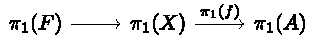
\includegraphics[width=0.95\linewidth,height=0.45\textheight,keepaspectratio]{graphic-17.pdf}\end{center}
\quad  \quad  
  
where $F\equiv\ker{f}$ is a set (because $f$ is covering) and thus $\pi_{1}(F)=1$.\par
 
% END S4.SS2.SSS0.P0.SPx1.p2
 
% BEGIN S4.SS2.SSS0.P0.SPx1.p3
 
We now have to show that these two operations are mutually inverse. Given a connected covering $f:X\to A$, the associated connected covering (by performing the two operations) is obtained as the pullback on the left, which can be rewritten as on the right.\par
  
\par  \quad   
\begin{center}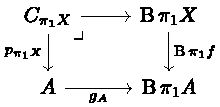
\includegraphics[width=0.95\linewidth,height=0.45\textheight,keepaspectratio]{graphic-18.pdf}\end{center}
 
\begin{center}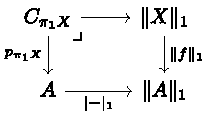
\includegraphics[width=0.95\linewidth,height=0.45\textheight,keepaspectratio]{graphic-19.pdf}\end{center}
 \quad  \quad  
  
The outer square of the diagram below commutes by naturality of the unit of the truncation, and we thus have a universal map $e:X\to C_{\pi_{1}X}$ such that\par
  
\par  \quad  
\begin{center}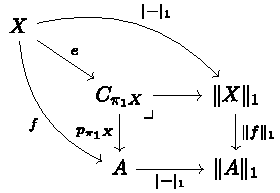
\includegraphics[width=0.95\linewidth,height=0.45\textheight,keepaspectratio]{graphic-20.pdf}\end{center}
\quad  \quad  
  
More explicitly,\par
  
\par  \quad  \[C_{\pi_{1}X}\quad\equiv\quad\Sigma(a:A).\Sigma(y:\|X\|_{1}).(|a|_{1}=\|f\|_{1}(y))\]\quad  \quad  
  
and $e(x)=(f(x),|x|_{1},\operatorname{refl}_{|f(x)|_{1}})$. Because the lower-left triangle commutes, $e$ is a map between types over $A$, and thus corresponds by Grothendieck duality (Theorem 1) to a family of fiberwise maps\par
  
\par  \quad  $\displaystyle e_{a}:\operatorname{fib}_{f}a$\quad  $\displaystyle\to\operatorname{fib}_{p_{\pi_{1}X}}a$\quad  \quad  
 
\par  \quad  $\displaystyle(x,p)$\quad  $\displaystyle\mapsto(f(x),|x|_{1},\operatorname{refl},p)$\quad  \quad  
  
indexed by $a:A$, with $p:a=f(x)$. Let us consider the case $a\equiv\star{}$. We have\par
  
\par  \quad  \[\operatorname{fib}_{p_{\pi_{1}X}}\star\quad\equiv\quad\Sigma(a:A).\Sigma(y:\|X\|_{1}).\Sigma(q:|a|_{1}=\|f\|_{1}(y)).(\star=a)\]\quad  \quad  
  
We can construct an inverse map to $e_{\star}$\par
  
\par  \quad  $\displaystyle e^{\prime}_{\star}:\operatorname{fib}_{p_{\pi_{1}X}}\star$\quad  $\displaystyle\to\operatorname{fib}_{f}\star$\quad  \quad  
 
\par  \quad  $\displaystyle(a,y,q,p)$\quad  $\displaystyle\mapsto(x,p\cdot\tilde{q})$\quad  \quad  
  
where we assume that $y=|x|_{1}$ because we are eliminating to $\operatorname{fib}_{f}\star$ which is a set (and thus a groupoid). Above, we have $p:|a|_{1}=\|f\|_{1}(x)$, which is equivalent to $\|a=f(x)\|_{0}$ (by [14, Theorem 7.3.12]) and we can thus suppose that $q=|\tilde{q}|_{0}$ with $\tilde{q}:a=f(x)$ because we are eliminating to a set. We have\par
  
\par  \quad  \[e^{\prime}\circ e(x,p)=(x,p\cdot\operatorname{refl})=(x,p)\]\quad  \quad  
  
Conversely,\par
  
\par  \quad  \[e\circ e^{\prime}(a,|x|_{1},|q|_{0},p)=e(x,p\cdot q)=(f(x),|x|_{1},\operatorname{refl},p\cdot q)\]\quad  \quad  
  
(we can suppose that the second and third arguments are truncations as above, because we are eliminating to a set). We thus have to show\par
  
\par  \quad  \[(f(x),|x|_{1},\operatorname{refl},p\cdot q)=(a,|x|_{1},|q|_{0},p)\]\quad  \quad  
  
with $p:\star=a$ and $q:a=f(x)$. Abstracting over $a$, we can suppose that $q$ is $\operatorname{refl}$ by J, and we conclude immediately.\par
 
% END S4.SS2.SSS0.P0.SPx1.p3
 
% BEGIN S4.SS2.SSS0.P0.SPx1.p4
 
Conversely, given a subgroup $i:G\hookrightarrow\pi_{1}A$, the associated subgroup (by performing the two transformations) is\par
  
\par  \quad  \[\pi_{1}(p_{G}):\pi_{1}C_{G}\to\pi_{1}A\]\quad  \quad  
  
we thus have to show that $\pi_{1}C_{G}=G$ and the map $\pi_{1}p_{G}=i$ (note that to be precise, we should identify the sources and the targets of the maps up to equality). We have a pullback square\par
  
\par  \quad  
\begin{center}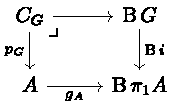
\includegraphics[width=0.95\linewidth,height=0.45\textheight,keepaspectratio]{graphic-21.pdf}\end{center}
\quad  \quad  
  
which can be extended as (see above)\par
  
\par  \quad  
\begin{center}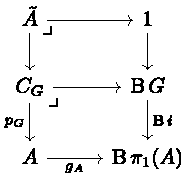
\includegraphics[width=0.95\linewidth,height=0.45\textheight,keepaspectratio]{graphic-22.pdf}\end{center}
\quad  \quad  
  
The map $C_{G}\to\operatorname{B}G$ is 1-connected because the fiber is $\tilde{A}$ which is 1-connected by Theorem 22. By [14, Lemma 7.5.14], it thus induces an equivalence $\|C_{G}\|_{1}\simeq\|\operatorname{B}G\|_{1}$, and thus $\pi_{1}(C_{G})=\pi_{1}(\operatorname{B}G)=G$. We should have the fact that $\pi_{1}p_{G}=i$ similarly, by applying $\pi_{1}$ to the above square (which is not anymore a pullback but remains commutative). $\hfill\blacktriangleleft$\par
 
% END S4.SS2.SSS0.P0.SPx1.p4
 
% BEGIN Thmtheorem37
 
\par\medskip\noindent\textbf{Example 37.}\par
 
% BEGIN Thmtheorem37.p1
 
Consider the case $A\equiv\operatorname{S}^{1}$. The associated Galois fibration is\par
  
\par  \quad  
\begin{center}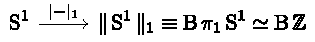
\includegraphics[width=0.95\linewidth,height=0.45\textheight,keepaspectratio]{graphic-23.pdf}\end{center}
\quad  \quad  
  
and is an equivalence, because $\operatorname{S}^{1}$ is a groupo\textbackslash{}̈operatorname\{i\}d. The subgroups of $\mathbb{Z}$ are of the form $i_{n}:\mathbb{Z}\to\mathbb{Z}$ with $i_{n}(k)=n\times k$ with $n>0$ or $i_{0}:0\to\mathbb{Z}$. And thus (connected) covering of the circle are obtained as pullbacks of the form\par
  
\par  \quad  
\begin{center}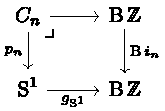
\includegraphics[width=0.95\linewidth,height=0.45\textheight,keepaspectratio]{graphic-24.pdf}\end{center}
\quad  \quad  
  
Since the lower arrow is an equivalence, the pullback $C_{n}$ is $\operatorname{B}\mathbb{Z}$, i.e. $\operatorname{S}^{1}$. And $p_{n}:\operatorname{S}^{1}\to\operatorname{S}^{1}$ is the pointed map of degree $n$, sending the loop to loopn.\par
 
% END Thmtheorem37.p1
 
% END Thmtheorem37
 
% END S4.SS2.SSS0.P0.SPx1
 
% END S4.SS2
 
% END S4



% BEGIN A1
 
\par\medskip\noindent\textbf{Appendix A Additional proofs}\par
 
% BEGIN A1.SS0.SSS0.P0.SPx1
 
\par\medskip\noindent\textbf{Proof of Lemma 21.}\par
 
% BEGIN A1.SS0.SSS0.P0.SPx1.p1
 
First, consider a property $P:(x,y:A)\to(p:x=y)\to\mathcal{U}$ such that $P\,x\,y\,p$ is a proposition for any $x,y:A$ and $p:x=y$. Since $A$ is pointed connected, the following are equivalent\par
  
\par\noindent  (i) 
% BEGIN A1.I1.i1.p1
 
$P\,x\,y\,p$ for any $x$, $y$ and $p$,\par
 
% END A1.I1.i1.p1
 
 
\par\noindent  (ii) 
% BEGIN A1.I1.i2.p1
 
$P\star\star\,p$ holds for any $p:\star=\star$.\par
 
% END A1.I1.i2.p1
 
  
Indeed, the second is a particular case of the first. Conversely, suppose (ii) holds, and that we are given $x$, $y$, and $p$. Since we want to show $P\,x\,y\,p$ which is a proposition, we can suppose given paths $p_{x}:\star=x$ and $p_{y}:\star=y$ because $A$ is connected, we then deduce that $P\,x\,y\,p$ holds from (ii) by transport.\par
 
% END A1.SS0.SSS0.P0.SPx1.p1
 
% BEGIN A1.SS0.SSS0.P0.SPx1.p2
 
Now, we have that $A$ is $(n{+}1)$-connected if and only if $x=y$ is $n$-connected for any $x,y:A$ (see Section 2) if and only if $\operatorname{\Omega}A$ is $n$-connected (by the preceding observation, based on the fact that being $n$-connected is a proposition [14, Theorem 7.1.10]) if and only if the pointing map $a=1\to A$ is $n$-connected (because we have $\operatorname{\Omega}A=\operatorname{fib}_{a}\star$). The reasoning is similar for the truncated version.\par
 
% END A1.SS0.SSS0.P0.SPx1.p2
 
% BEGIN A1.SS0.SSS0.P0.SPx1.p3
 
An alternative proof for the connected case can be found in [14, Lemma 7.5.11]. $\hfill\blacktriangleleft$\par
 
% END A1.SS0.SSS0.P0.SPx1.p3
 
% END A1.SS0.SSS0.P0.SPx1
 
% BEGIN A1.SS0.SSS0.P0.SPx2
 
\par\medskip\noindent\textbf{Proof of Proposition 25.}\par
 
% BEGIN A1.SS0.SSS0.P0.SPx2.p1
 
Since $\tilde{A}$ is $(n{+}1)$-connected by Theorem 22, we have $\pi_{i}(\tilde{A})=1$ for $i\leq n+1$ [14, Lemma 8.3.2]. For $i>n+1$, this is a consequence of the long exact sequence induced by the fiber sequence of Theorem 24, see [14, Theorem 8.4.6]:\par
  
\par  \quad  
\begin{center}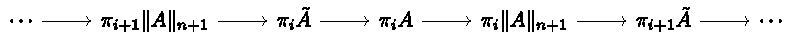
\includegraphics[width=0.95\linewidth,height=0.45\textheight,keepaspectratio]{graphic-37.pdf}\end{center}
\quad  \quad  
  
We have $\pi_{i}\|A\|_{n+1}=1$ and the short exact sequence\par
  
\par  \quad  
\begin{center}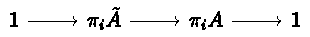
\includegraphics[width=0.95\linewidth,height=0.45\textheight,keepaspectratio]{graphic-38.pdf}\end{center}
\quad  \quad  
  
shows that $\pi_{i}\tilde{A}=\pi_{i}A$. $\hfill\blacktriangleleft$\par
 
% END A1.SS0.SSS0.P0.SPx2.p1
 
% BEGIN A1.SS0.SSS0.P0.SPx2.p2
 
The following two lemmas (Lemma 41 and Lemma 42) are used in the subsequent proof of Lemma 35:\par
 
% END A1.SS0.SSS0.P0.SPx2.p2
 
% BEGIN Thmtheorem41
 
\par\medskip\noindent\textbf{Lemma 41.}\par
 
% BEGIN Thmtheorem41.p1
 
Suppose given an injective group morphism $f:G\to H$. Then $\ker\operatorname{B}f$ is a set.\par
 
% END Thmtheorem41.p1
 
% END Thmtheorem41
 
% END A1.SS0.SSS0.P0.SPx2
 
% BEGIN A1.SS0.SSS0.P0.SPx3
 
\par\medskip\noindent\textbf{Proof.}\par
 
% BEGIN A1.SS0.SSS0.P0.SPx3.p1
 
We have, by definition:\par
  
\par  \quad  \[\ker\operatorname{B}f\quad\equiv\quad\Sigma(x:\operatorname{B}G).(\star=\operatorname{B}f(x))\]\quad  \quad  
  
Given $(x,p):\ker\operatorname{B}f$, we want to prove that the loop space\par
  
\par  \quad  \[(x,p)=(x,p)\]\quad  \quad  
  
is a proposition (this is enough to show that $\ker\operatorname{B}f$ is set by [14, Theorem 7.2.1]). Since $\operatorname{B}G$ is connected, we merely have a path $q:\star=x$. Since being a proposition for the loop space is a proposition, we can suppose given such a path $q$, and by path induction it is enough to prove that\par
  
\par  \quad  \[(\star,p)=(\star,p)\]\quad  \quad  
  
is a proposition, with $p:\Omega\operatorname{B}H$. By the characterization of paths in $\Sigma$-types [14, Theorem 2.7.2] and transport along identity types [14, Theorem 2.11.3], the above type is equivalent to\par
  
\par  \quad  \[\Sigma(a:\star=\star).(p\cdot\operatorname{B}f^{=}(a)=p)\]\quad  \quad  
  
We then have the following chain of equivalences:\par
  
\par  \quad  $\displaystyle\Sigma(a:\star=\star).$\quad  $\displaystyle(p\cdot\operatorname{B}f^{=}(a)=p)$\quad  \quad  
 
\par  \quad  \quad  $\displaystyle=\Sigma(a:\star=\star).(\operatorname{B}f^{=}(a)=\operatorname{refl}_{\operatorname{B}f(\star)})$\quad  by left simplification by $p$\quad  \quad  
 
\par  \quad  \quad  $\displaystyle=\Sigma(a:G).(f(a)=_{H}1_{H})$\quad  we use $\Omega\operatorname{B}G=G$ and $\Omega\operatorname{B}H=H$\quad  \quad  
 
\par  \quad  \quad  $\displaystyle=\Sigma(a:G).(f(a)=_{H}f(1_{G}))$\quad  because $f$ is a morphism\quad  \quad  
 
\par  \quad  \quad  $\displaystyle=\Sigma(a:G).(a=_{G}1_{G})$\quad  because $f$ is injective\quad  \quad  
  
This latter type is contractible [14, Lemma 3.11.8] and is thus a proposition. $\hfill\blacktriangleleft$\par
 
% END A1.SS0.SSS0.P0.SPx3.p1
 
% BEGIN Thmtheorem42
 
\par\medskip\noindent\textbf{Lemma 42.}\par
 
% BEGIN Thmtheorem42.p1
 
Suppose given a group morphism $i:H\to G$ and a function $f:G\to X$, where $X$ is a set, and $f$ is invariant by the action of $H$ on $G$ induced by right multiplication, and such that $\operatorname{fib}_{f}x$ is the group $H$ equipped with its canonical action on itself for every $x:X$. Then $X=G/H$.\par
 
% END Thmtheorem42.p1
 
% END Thmtheorem42
 
% END A1.SS0.SSS0.P0.SPx3
 
% BEGIN A1.SS0.SSS0.P0.SPx4
 
\par\medskip\noindent\textbf{Proof.}\par
 
% BEGIN A1.SS0.SSS0.P0.SPx4.p1
 
Recall that the quotient is the set truncation of the homotopy coequalizer\par
  
\par  \quad  
\begin{center}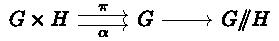
\includegraphics[width=0.95\linewidth,height=0.45\textheight,keepaspectratio]{graphic-39.pdf}\end{center}
\quad  \quad  
  
with $\pi$ the first projection and $\alpha$ the right action of $H$ on $G$ (we have $\alpha(a,b)\equiv a\times i(b)$), i.e. $G/H=\|G{/\!\!/}H\|_{0}$. Otherwise said, $G/H$ satisfies the same universal property as the above equalizer but restricted to sets. Our aim is now to show that $f:G\to X$ satisfies this universal property. The hypothesis that $f$ is invariant under the action of $H$ precisely means that it coequalizes the two maps. Suppose given another coequalizing map $g:G\to Y$ with $Y$ a set. We need to show that there exists a unique map $h:X\to Y$ such that $h\circ f=g$:\par
  
\par  \quad  
\begin{center}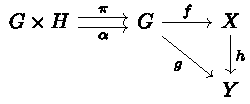
\includegraphics[width=0.95\linewidth,height=0.45\textheight,keepaspectratio]{graphic-40.pdf}\end{center}
\quad  \quad  
  
The existence of such an $h$ is implied by the fact that we have, for every $x:X$, an element $a:\operatorname{fib}_{f}x$ such that for every element $b:\operatorname{fib}_{f}x$, we have $g(a)=g(b)$. This condition is satisfied. Indeed, under the identification of $\operatorname{fib}_{f}x$ with $H$, we can take $a$ to be the neutral element of $H$, and the fact that the action of $H$ on itself is transitive and that $g$ preserves this action ensures that any other image will be equal to this one. $\hfill\blacktriangleleft$\par
 
% END A1.SS0.SSS0.P0.SPx4.p1
 
% END A1.SS0.SSS0.P0.SPx4
 
% BEGIN A1.SS0.SSS0.P0.SPx5
 
\par\medskip\noindent\textbf{Proof of Lemma 35.}\par
 
% BEGIN A1.SS0.SSS0.P0.SPx5.p1
 
Recall that we have\par
  
\par  \quad  \[\ker\operatorname{B}i\quad\equiv\quad\Sigma(x:\operatorname{B}H).(\star=\operatorname{B}i\,x)\]\quad  \quad  
  
We define a map\par
  
\par  \quad  \[f:G\to\ker\operatorname{B}i\]\quad  \quad  
  
by $f(a)\equiv(\star,p_{a})$ for $a:G$ corresponding to a path $p_{a}:\star=\star$ in $\operatorname{B}G$. The fibers of this map are\par
  
\par  \quad  $\displaystyle\operatorname{fib}_{f}(x,p)$\quad  $\displaystyle\equiv\Sigma(a:G).((x,p)=(\star,p_{a}))$\quad  \quad  
 
\par  \quad  \quad  $\displaystyle=\Sigma(a:G).\Sigma(q:x=\star).(p\cdot(\operatorname{B}i)^{=}(q)=p_{a})$\quad  \quad  
  
In particular, for $x\equiv\star$, we have $p\equiv p_{b}$ for some $b:G$ and the fiber is\par
  
\par  \quad  $\displaystyle\operatorname{fib}_{f}(\star,p_{b})$\quad  $\displaystyle=\Sigma(a:G).\Sigma(c:H).(b\times i(c)=a)$\quad  \quad  
 
\par  \quad  \quad  $\displaystyle=\Sigma(c:H).\Sigma(a:G).(b\times i(c)=a)$\quad  \quad  
 
\par  \quad  \quad  $\displaystyle=H$\quad  \quad  
  
Since $\operatorname{B}H$ is connected, we can deduce that $\operatorname{fib}_{f}(x,p)$ merely is $H$ for any $(x,p):\ker\operatorname{B}i$. Furthermore, $f$ is invariant under the action of $H$. Given $a:G$ and $b:H$, we have\par
  
\par  \quad  $\displaystyle f(b\cdot a)$\quad  $\displaystyle\equiv(\star,p_{(b\cdot a)})$\quad  \quad  
 
\par  \quad  \quad  $\displaystyle\equiv(\star,p_{(a\times i(b))})$\quad  \quad  
 
\par  \quad  \quad  $\displaystyle\equiv(\star,p_{a}\cdot p_{i(b)})$\quad  \quad  
 
\par  \quad  \quad  $\displaystyle=(\star,p_{a})$\quad  by transport along $p_{i(b)}^{-1}$ in $\lambda x.(\star=\operatorname{B}i(x))$ ([14, Th. 2.11.3])\quad  \quad  
 
\par  \quad  \quad  $\displaystyle\equiv f(a)$\quad  \quad  
  
Finally, by Lemma 41, $\ker\operatorname{B}i$ is a set since $i$ is injective. By Lemma 42, we deduce that $\ker\operatorname{B}i$ merely is $G/H$. $\hfill\blacktriangleleft$\par
 
% END A1.SS0.SSS0.P0.SPx5.p1
 
% END A1.SS0.SSS0.P0.SPx5
 
% END A1


% BEGIN bib
 
\par\medskip\noindent\textbf{References}\par
  
\par\noindent  [1]  Marc Bezem, Ulrik Buchholtz, Pierre Cagne, Bjørn Ian Dundas, and Daniel R. Grayson.  Symmetry.  URL: https://github.com/UniMath/SymmetryBook.  
 
\par\noindent  [2]  Ulrik Buchholtz and Egbert Rijke.  The long exact sequence of homotopy $n$-groups.  Mathematical Structures in Computer Science, 33(8):679–687, 2023.  doi:10.1017/S0960129523000038.  
 
\par\noindent  [3]  Camil Champin, Samuel Mimram, and Émile Oleon.  Delooping Generated Groups in Homotopy Type Theory.  In 9th International Conference on Formal Structures for Computation and Deduction (FSCD 2024), volume 299 of LIPIcs, pages 6:1–6:20. Schloss Dagstuhl, 2024.  doi:10.4230/LIPIcs.FSCD.2024.6.  
 
\par\noindent  [4]  Camil Champin, Samuel Mimram, and Émile Oleon.  Delooping presented groups in homotopy type theory.  Submitted, 2025.  arXiv:2405.03264.  
 
\par\noindent  [5]  Henri Paul de Saint Gervais.  Analysis situs: Variété dodécaédrique de poincaré, 2014.  URL: https://analysis-situs.math.cnrs.fr/-Variete-dodecaedrique-de-Poincare-.html.  
 
\par\noindent  [6]  Michel Demazure and Pierre Gabriel.  Groupes Algébriques, Tome 1.  North-Holland Publishing Company, 1970.  
 
\par\noindent  [7]  Allen Hatcher.  Algebraic topology.  Cambridge University Press, 2009.  
 
\par\noindent  [8]  Kuen-Bang Hou and Robert Harper.  Covering spaces in homotopy type theory.  In 22nd International Conference on Types for Proofs and Programs (TYPES 2016), pages 11–1. Schloss Dagstuhl – Leibniz-Zentrum für Informatik, 2018.  doi:10.4230/LIPIcs.TYPES.2016.11.  
 
\par\noindent  [9]  Samuel Mimram and Emile Oleon.  Delooping cyclic groups with lens spaces in homotopy type theory.  In Proceedings of the 39th Annual ACM/IEEE Symposium on Logic in Computer Science, LICS’24, New York, 2024. Association for Computing Machinery.  doi:10.1145/3661814.3662077.  
 
\par\noindent  [10]  Samuel Mimram and Émile Oleon.  Hypercubical manifolds in homotopy type theory.  Submitted, 2025.  doi:10.48550/arXiv.2506.19402.  
 
\par\noindent  [11]  Henri Poincaré.  Cinquième complément à l’analysis situs.  Rendiconti del Circolo Matematico di Palermo (1884-1940), 18(1):45–110, 1904.  
 
\par\noindent  [12]  Egbert Rijke.  Introduction to Homotopy Type Theory.  Cambridge Studies in Advanced Mathematics. Cambridge University Press, 2025.  
 
\par\noindent  [13]  Hugo Salou.  Classifying covering types in Agda, 2025.  URL: https://github.com/hugo-s29/classifying-covering-types-agda.  
 
\par\noindent  [14]  The Univalent Foundations Program.  Homotopy Type Theory: Univalent Foundations of Mathematics.  https://homotopytypetheory.org/book, Institute for Advanced Study, 2013.  
 
\par\noindent  [15]  Vladimir Voevodsky.  A very short note on homotopy $\lambda$-calculus.  Unpublished note, 2006.  
 
\par\noindent  [16]  David Wärn.  Eilenberg–Maclane spaces and stabilisation in homotopy type theory.  Journal of Homotopy and Related Structures, 18(2):357–368, 2023.  doi:10.1007/s40062-023-00330-5.  
 
\par\noindent  [17]  Jelle Wemmenhove, Cosmin Manea, and Jim Portegies.  Classification of covering spaces and canonical change of basepoint.  Preprint, 2024.  doi:10.48550/arXiv.2409.15351.  
  
% END bib

\end{document}
